\begin{center}
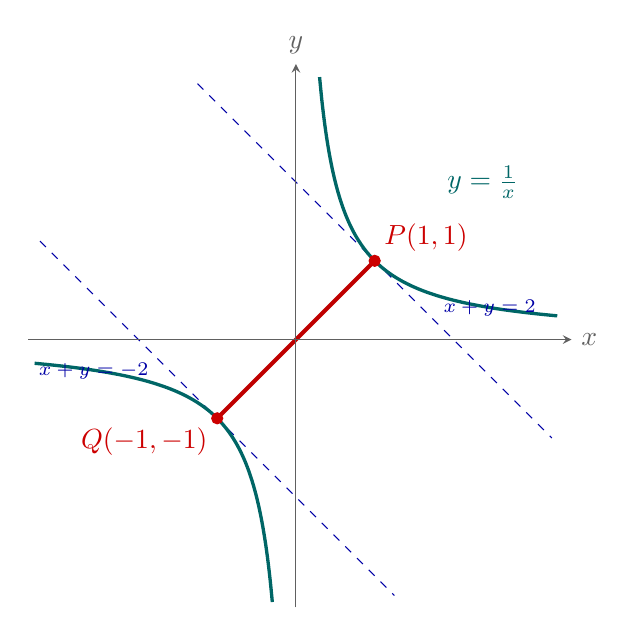
\begin{tikzpicture}[x=1.00cm,y=1.00cm,>=stealth]
  \begin{scope}
    \clip (-3.35,-3.35) rectangle (3.35,3.35);
    \draw[dashed,blue!65!black,thin] (-1.25,3.25)--(3.25,-1.25);
    \draw[dashed,blue!65!black,thin] (-3.25,1.25)--(1.25,-3.25);
    \draw[very thick,teal!80!black,domain=0.30:3.32,samples=110,smooth,variable=\t] plot ({\t},{1/\t});
    \draw[very thick,teal!80!black,domain=0.30:3.32,samples=110,smooth,variable=\t] plot ({-\t},{-1/\t});
    \draw[line width=1.5pt,red!75!black] (-1,-1)--(1,1);
  \end{scope}
  \draw[->,gray!75!black] (-3.4,0)--(3.5,0) node[right] {$x$};
  \draw[->,gray!75!black] (0,-3.4)--(0,3.5) node[above] {$y$};
  \filldraw[red!80!black] (1,1) circle (2pt) node[above right] {$P(1,1)$};
  \filldraw[red!80!black] (-1,-1) circle (2pt) node[below left] {$Q(-1,-1)$};
  \node[blue!65!black,anchor=west] at (1.75,0.4) {\scriptsize $x+y=2$};
  \node[blue!65!black,anchor=east] at (-1.75,-0.4) {\scriptsize $x+y=-2$};
  \node[teal!80!black,anchor=west] at (1.8,2.0) {$y=\frac1x$};
\end{tikzpicture}

{\footnotesize 图：以 $k=1$ 为例。两条虚线把两支曲线隔开，红色线段是最短的连接线段，长度为 $2\sqrt2$。}
\end{center}
